\chapter{Pruebas}

\textit{``Los tests en el desarrollo guiado por pruebas (TDD) son los dientes de un engranaje.
Una vez que se desarrolla un test completamente funcional, es seguro que este va a funcionar por y
para siempre.''~\cite{beck2003test}
}

\section{Metodología TDD}
Tal y como se había comentado en el capítulo anterior, el periodo de codificación de cada una de las
funcionalidades ha sido posterior a una fase de creación de \textit{suite de tests automatizados}. 
Este \textit{modus operandi}
es propio de la metodología \textit{Test Driven Development} (TDD), práctica que se ha usado por desarrolladores durante
decadas y que ha ido ganando popularidad como una de las prácticas principales de
la metodología \textit{Extreme Programming}~\cite{1510569}.

\begin{figure}[H]
    \centering
    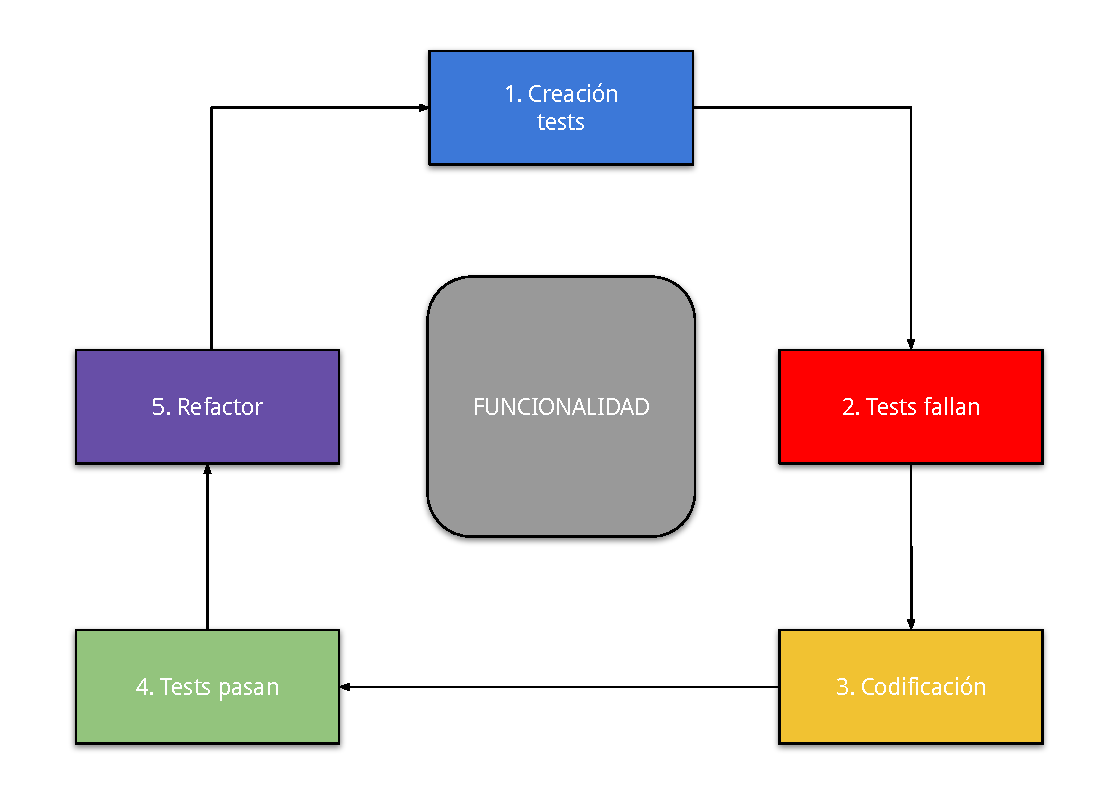
\includegraphics[scale=0.7]{images/tdd_diagram.pdf}
    \caption{Diagrama de flujo de la metodología TDD}
    \label{fig:tdd-diagram}
\end{figure}

La elección de la arquitectura hexagonal \textit{Clean Architecture} en el proyecto es un aspecto que
facilita notablemente la implementación de la metodología en el proyecto, permitiendo
abstraer completamente los test para poder reutilizarlos incluso en otros casos de uso.

Las pautas de esta metodología sugieren un diagrama de flujo similar al de la \autoref{fig:tdd-diagram},
este flujo de estados se ha aplicado a todas las funcionalidades (\textit{features}) del
proyecto:

\begin{enumerate}
    \item De cara a integrar una nueva funcionalidad en el proyecto, se desarrolla una
    \textit{suite de tests}, obteniendo una idea central y unas pautas más claras de la funcionalidad a desarrollar.
    \item El siguiente paso consiste en ejecutar los tests. De forma evidente se obtiene 
    una serie de resultados fallidos, ya que aún no se ha desarrollado la funcionalidad.
    Las pruebas deben de testar funciones lo más concretas y triviales posibles, además de ser
    completamente independientes unas de otras.
    \item En este momento se desarrolla la funcionalidad, dividida por las capas
    ya comentadas en el anterior capítulo.
    \item Conforme se va desarrollando la funcionalidad la ejecución de los tests
    van adquiriendo valores exitosos. De este modo, se asegura que la las porciones de código desarrolladas
    puedan contener el mínimo número de \textit{bugs}.
    \item Una vez la ejecución de los tests de la funcionalidad tiene ausencia de errores, 
    se procede a la \textit{refactorización} del código (desde cambios de nombres de variables
    hasta desechar posibles elementos innecesarios). Estas sucesivas \textit{refactorizaciones}
    favorecen que el producto esté mantenido de forma constante.
 \end{enumerate}

 Ya enumerados estos pasos, se llega a la conclusión de que la idea central, que alberga esta 
 metodología \textit{TDD}, no se resume como el simple hecho de \textit{testear antes de escribir código}, sino un
 proceso capaz de:

 \begin{itemize}
     \item[$\bullet$] Explorar y comprender mejor la problemática central de la solución antes de comenzar con
     su implementación.
     \item[$\bullet$] Detectar y anticiparse frente a  posibles excepciones o problemas que
     puedan surgir durante el desarrollo.
     \item[$\bullet$] Detectar posibles actualizaciones de requisitos en base a la complejidad
     de una determinada prueba \textit{(retrospectiva)}.
 \end{itemize}

 En la práctica, resulta realmente extensa la cantidad de tipos de pruebas que se pueden emplear para testar una
 solución \textit{software}. \textit{Flutter}, como cualquier otro \textit{framework} de desarrollo, presenta
 numerosas herramientas para favorecer y aligerar esta tarea. Los tipos de pruebas más recurrentes que presenta este entorno
 son: tests de \textit{widgets}, \textit{golden}, \textit{end-to-end}, 
 \textit{integración} y \textit{unitarios}.
 
 Con el fin de obtener la mayor \textit{cobertura de código} posible en el aplicativo, se ha optado por el uso de estos
 tres últimos, además de ser plenamente complementarios. En los siguientes apartados se introducirán y explicarán su uso en el sistema.

 En cuanto al entorno y herramientas que se han empleado para la realización de las pruebas
 son las proporcionadas por el \textit{IDE} de desarrollo \textit{Visual Studio Code}, mediante su modo
 \textit{testing} (\textit{flutter test}).

 Gracias a este entorno se han podido ejecutar todas las baterías de pruebas,
 de forma individual como completa. 

 \subsection{Pruebas unitarias}
 Los tests unitarios son una parte fundamental de cualquier desarrollo
 de \textit{software}, pues son tests automatizados que aseguran el correcto
 funcionamiento de determinados componentes, llamados individualmente como \textit{unidad}.

 Según el volumen ``\textit{Unit Testing: Principles, Practices, and Patterns}'' de \textit{Vladimir Khorikov} (pp. 21) \cite{khorikov2020unit}, un test se considera unitario cuando reúne estas tres características:
 \begin{itemize}
     \item[$\bullet$] Verifica una única funcionalidad.
     \item[$\bullet$] Se crea de forma trivial y rápida.
     \item[$\bullet$] Se desarrolla de forma independiente.
 \end{itemize}

 En este proyecto se han realizado tests de la totalidad de las clases \textit{modelo} y \textit{entidad}, ya que
 son las que va a emplear las funcionalidades del aplicativo final. Entre los más importantes se destaca, como
 no podía ser de otra forma, el \textit{modelo} de la entidad
 \textit{nonograma}, ya que es la que está presente en la mayoría de casos de uso de la solución.

 Mediante el paquete \textit{flutter\_test} se testea un objeto del
 modelo \textit{Nonograma}. Este objeto se instancia en un método \textit{setUp()} con ciertos valores 
 arbitrarios y se testean ciertas casuísticas en forma de \textit{tests}, 
 todos ellos comprendidos en un método \textit{main()}
 que se encarga de ejecutarlos.
 Todos estos \textit{tests} pueden ``agruparse'' en forma \textit{groups}, en el caso de que exista una correlación
 entre cada uno de ellos.

 Algunas de las pruebas unitarias que se han implementado relacionados con el modelo \textit{Nonograma}
 han verificado:

 \begin{itemize}
    \item[$\bullet$] El nombre completo (comprobar que no sea vacío y no contenga carácteres especiales).
    \item[$\bullet$] El número de celdas correctas (comprobar que esté comprendido en el array).
    \item[$\bullet$] Las dimensiones (número de filas y columnas con un formato concreto: 5x5, 10x10,...).
    \item[$\bullet$] La resolución de un nivel concreto (el \textit{nonograma} de la solución sea igual al original).
    \item[$\bullet$] El identificador del \textit{nonograma} sea único con respecto a los otros \textit{nonogramas}.
 \end{itemize}

 \subsection{Pruebas de integración}
 Siguiendo el mismo ejemplar anteriormente citado, un test de \textit{integración} es aquel que no reúne ninguna
 de las tres características, previamente enumeradas, propias de los \textit{tests unitarios}.
 Estos tipos de test cubren las porciones de código relacionadas con los controladores y
 lógicas de negocio.

 En el caso de este aplicativo, las pruebas de integración se encargarán de cubrir y testar todos los posibles comportamientos
 que comprenden los manejadores de estados, las clases \textit{BLoC}.

 En estos tipos de pruebas se inicializa el \textit{BLoC} a probar mediante
 el método \textit{setUp()} y se testea la sucesión de \textit{estados} que emite este mismo
 objeto frente a un determinado \textit{evento}. Toda esta sucesión de \textit{estados} se definen en un \textit{array}
 y se comparan con la cadena de \textit{estados} esperada mediante el método \textit{expect()}.

 Además, los \textit{BLoCs} pueden interactuar con servicios externos a usar por el aplicativo como \textit{bases de datos locales y remotas},
 \textit{pasarelas de pago}, \textit{librerías de terceros}... Y aquí entra en juego un término ampliamente conocido en el mundo del  \textit{testing},
 los \textit{Mocks}.

 Los \textit{mocks} son objetos de ``prueba'' que simulan o imitan ciertos comportamientos
 de objetos reales en un entorno controlado. Con estos tipos de objetos se pueden simular
 todos las casuísticas de una determinado caso de uso, desde excepciones y fallos hasta situaciones
 ideales.
 Todas estos casos en el patrón \textit{BLoC} se pueden traducir en forma de estados.

 El uso de estos \textit{mocks} permitirá el uso de los servicios a emplear por \textit{BLoC} sin
 su concreta implementación en un entorno de \textit{producción}.
 
 Mediante la librería externa \textit{mockito} se permitirá incorporar este tipo de objetos
 en el aplicativo. Cada servicio a simular debe de
 extender de la clase \textit{Mock}, proporcionado por el propio paquete \textit{mockito}.
 En él se inicializan, mediante el método \textit{setUp()}, el \textit{BLoC} a probar junto con
 los servicios a simular mediante \textit{Mocks}.

 Algunas de las pruebas de integración de interés en el aplicativo han verificado las
 siguientes funcionalidades de \textit{BLoCs} relativos a \textit{nonogramas}:

 \begin{itemize}
    \item[$\bullet$] Recibir la lista de \textit{nonogramas} en línea sin errores.
    \item[$\bullet$] Al ``pintar'' una celda comprobar que la celda está dentro de las celdas seleccionadas.
    \item[$\bullet$] La publicación de un \textit{nonograma} concreto sin errores.
    \item[$\bullet$] Comprobar si existe el progreso de la resolución de un nivel si está la opción
    de autoguardado activado.  
    \item[$\bullet$] Al seleccionar la última celda correcta del nivel comprobar que el \textit{nonograma}
    aparece como \textit{resuelto}. 
 \end{itemize}

 \subsection{Pruebas end-to-end}
 Las \textit{pruebas end-to-end}, son las pruebas finales y verifican que
 toda la experiencia de usuario es satisfactoria en un entorno con los servicios reales
 y en conexión y disponibles para el aplicativo. En este momento se definirá si una
 determinada funcionalidad estará preparada para su inclusión en el sistema,
 o en su defecto, requiere un ajuste en el diseño.

 La representación de estos tres tipos de pruebas en el aplicativo se refleja en la \autoref{fig:test-diagram}, en
 esta se puede observar su alcance en este proyecto.

 \begin{figure}[H]
    \centering
    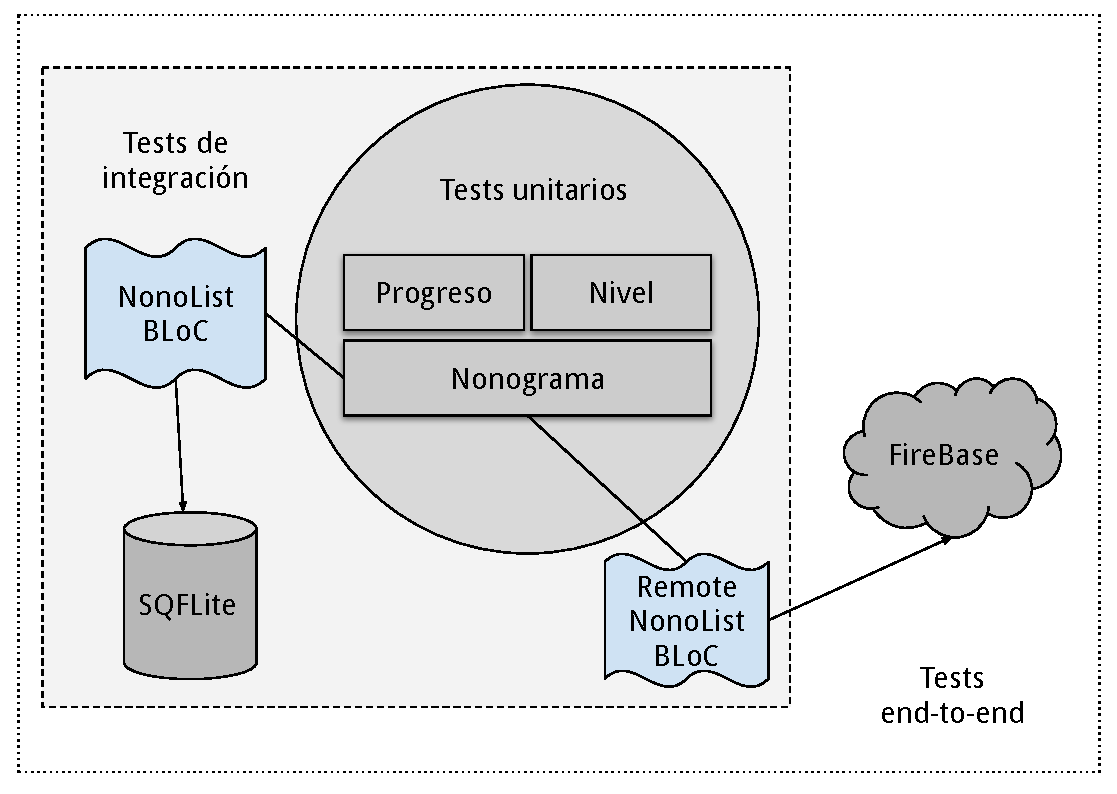
\includegraphics[scale=0.5]{images/testdiagram.pdf}
    \caption{Diagrama de los tipos de pruebas en el aplicativo}
    \label{fig:test-diagram}
\end{figure}